\documentclass[10pt,english]{beamer}
%\documentclass[english,handout]{beamer} % For handouts
\usetheme[progressbar=frametitle,block=fill]{metropolis} %numbering=none

%%% USEFUL PACKAGES
%\usepackage{showframe} % For debugging positioning
\usepackage{etex} % If too many packages
% Encoding and language
\usepackage[utf8]{inputenc}
\usepackage{babel}
\usepackage{amsmath, amssymb}
\usepackage{natbib}
%\usepackage{booktabs}
%\usepackage{algorithmic}
\usepackage{algorithm}
\usepackage{caption}
%\usepackage{animate} % Animations
\usepackage{bm} % Bold math
\usepackage{bbm}
%\usepackage{url}
%\usepackage{pifont}
%\usepackage{ulem} % Used for strikeouts \sout
%\usepackage{stackengine}
%\usepackage{enumitem}
%\setlist[description]{leftmargin=\parindent,labelindent=\parindent}
%\usepackage{colortbl} % Used for colored rows in tables


%%% GRAPHICS
\usepackage{graphicx}
\graphicspath{{./figs/}}


%%% COLORS
\setbeamercolor{background canvas}{bg=white}
\def\BlankFrame{
	\bgroup
	%\pdfpageheight 29.7cm
	\setbeamercolor{background canvas}{bg=}
	\begin{frame}[plain]
	\end{frame}
	%\makeatletter
	%\pdfpageheight \beamer@paperheight
	%\makeatother
	\egroup}

\usepackage{xcolor}
\definecolor{DarkGreen}{HTML}{00B200}
\definecolor{LightBlue}{HTML}{0090D9}
\definecolor{gold}{rgb}{.812,.710,.231}
% Text markup
%\setbeamercolor{alerted text}{fg=red}
\newcommand{\blue}[1]{\textcolor{blue}{#1}}
\newcommand{\red}[1]{\textcolor{red}{#1}}
\newcommand{\grey}[1]{\textcolor{gray}{#1}}
\newcommand{\orange}[1]{\textcolor{mLightBrown}{#1}}
\newcommand\myheading[1]{\textbf{#1}}
\newcommand\myemph[1]{\underline{\emph{#1}}}
\newcommand\textexample[1]{\textit{\textbf{#1}}}

%%% SPACING
\newcommand\vws[1][1]{\vspace{#1\baselineskip}} % vertical white space
%\newcommand\strt[1][1.5ex]{\rule[-.05\baselineskip]{0pt}{#1}} % strut
\newcommand\strt[2]{\rule[-#1ex]{0pt}{#2ex}} % strut
\newcommand\Hrule{\vspace{1ex} \hrule \vspace{1ex}} % Horisontal rule with some space after

%%% MISC
\newcommand\articleref[4]{\noindent\begin{minipage}[t]{0.04\textwidth}
		\vspace{0pt} 
		\pgfuseimage{beamericonarticle}
	\end{minipage}%
	\begin{minipage}[t]{0.96\textwidth}
		\vspace{0pt}
		#1. \textbf{#2.} \textit{#3}, #4.
	\end{minipage}}

%%% METROPOLIS THEME SPECIFIC
\makeatletter
\setlength{\metropolis@progressonsectionpage@linewidth}{1pt}
\makeatother
%\setbeamercolor{progress bar}{fg=red,bg=red!50}


%%% TEXTPOS
\usepackage[absolute,overlay]{textpos} % option showboxes is useful in draft mode
\setlength{\TPHorizModule}{\paperwidth}
\setlength{\TPVertModule}{\paperheight}
\textblockorigin{0pt}{10mm} % start everything at top-left, below gray 


%%% TIKZ/PGFPLOTS
\usepackage{tikz}
\usetikzlibrary{arrows,positioning,calc,shapes.geometric}
%\usetikzlibrary{arrows,calc,shapes.geometric,decorations.pathmorphing,backgrounds,positioning,fit,petri,decorations.pathreplacing}
%\usepackage{pgfplots}
%\pgfplotsset{compat = 1.3}


%%% BLOCKS AND BOXES
% Changing colors of blocks
%\setbeamercolor{block title alerted}{bg=UURed,fg=palette primary.fg}
%\setbeamercolor{block body alerted}{bg=UURed!15}
\setbeamercolor{block title alerted}{bg=mLightBrown,fg=palette primary.fg}
\setbeamercolor{block body alerted}{bg=mLightBrown!15}
%\setbeamercolor{block title example}{bg=UUGreen,fg=palette primary.fg}
%\setbeamercolor{block body example}{bg=UUGreen!10}
% \mybox is a rectangular box
\usepackage{boxedminipage}
\setlength\fboxrule{2pt}
\setlength\fboxsep{2\fboxsep}
\newcommand\mybox[3][\textwidth]{
  {\color{#2}
    \begin{boxedminipage}{#1}
      {\color{palette primary.bg} #3}
    \end{boxedminipage}}%
}   
\usepackage{tcolorbox}
\tcbset{arc=1mm,grow to left by=3mm,grow to right by=3mm,left=2mm}
%\newenvironment{redbox}{%
%	\begin{tcolorbox}[colback=UURed!15,colframe=UURed]}{%
%	\end{tcolorbox}}
%\newenvironment{greenbox}{%
%	\begin{tcolorbox}[colback=UUGreen!15,colframe=UUGreen]}{%
%	\end{tcolorbox}}
\newenvironment{redbox}{%
	\begin{tcolorbox}[colback=red!15,colframe=red]}{%
	\end{tcolorbox}}
\newenvironment{greenbox}{%
	\begin{tcolorbox}[colback=DarkGreen!15,colframe=DarkGreen]}{%
	\end{tcolorbox}}
\newenvironment{graybox}{%
	\begin{tcolorbox}[colback=mDarkTeal!5,colframe=mDarkTeal]}{%
	\end{tcolorbox}}
\newenvironment{orangebox}{%
\begin{tcolorbox}[colback=mLightBrown!15,colframe=mLightBrown]}{%
	\end{tcolorbox}}
\newenvironment{bwbox}{%
	\begin{tcolorbox}[colback=white,colframe=black]}{%
\end{tcolorbox}}
\newenvironment{bluebox}{%
	\begin{tcolorbox}[colback=LightBlue!15,colframe=LightBlue]}{%
\end{tcolorbox}}


%%%%%%%%% NEW MACROS

\newcommand\imp[1]{\alert{\textbf{#1}}}
\newcommand\bfit[1]{\textbf{\textit{#1}}}
\newcommand\good{\color{DarkGreen}{$\blacktriangle$}} % used in lists
\newcommand\bad{\color{red}{$\blacktriangledown$}} % used in lists


\RequirePackage{amsmath, amssymb}
\RequirePackage{bbm}
%\RequirePackage{newtxmath}


% Convenience macro for referring to data source
\newcommand\sourceurl[2]{\small \grey{Data from \href{#1}{#2}}}

% Abbreviations
\RequirePackage{xspace}
\newcommand\pdf{pdf\xspace}
\newcommand\ifft{iff\xspace}
\newcommand\ex{\textbf{ex)}\xspace}

% General time series notation
\newcommand\T{n}  % Length of time series
\newcommand\rtheta{{\red{\theta}}}  % Parameter (color coded)
\newcommand\rthetah{{\red{\widehat\theta}}}  % Estimate (color coded)

% Neural netowkrs
\newcommand\h{\mathbf{h}} % Hidden state variable
\newcommand\zz{\mathbf{z}} % Generic input (vector)

% For OLS/AR
\newcommand\noise{\varepsilon}  % This is the noise in AR, but should it be the same as measurement noise in SSM?
\newcommand\noisevar{\sigma^2_\noise}
\newcommand\noisevarhat{\widehat\sigma^2_\noise}
\newcommand\X{\Phi}
\newcommand\y{\mathbf{y}}
\newcommand\bphi{\bm\phi}

% State space models
\newcommand\z{\alpha}  % State vector, general SSM
\newcommand{\obsnoise}{\varepsilon}
\newcommand{\statenoise}{\eta}
\newcommand{\varobs}{\sigma^2_{\varepsilon}}
\newcommand{\varstate}{\sigma^2_{\eta}}
% For structural time series
\newcommand{\trendnoise}{\zeta}
\newcommand{\seasnoise}{\omega}
\newcommand{\vartrend}{\sigma^2_{\trendnoise}}
\newcommand{\varseas}{\sigma^2_{\seasnoise}}

%
\newcommand\FF{T}
\newcommand\GG{R}
\newcommand\HH{Z}
\newcommand{\covobs}{\sigma_\epsilon^2}
\newcommand{\covstate}{Q}
\newcommand\initmean{a_1}
\newcommand\initcov{P_1}
% Kalman filter
\newcommand{\zpart}[2]{\z_{#1}^{#2}}
\newcommand{\wgt}[2]{\omega_{#1}^{#2}}
\newcommand{\wgtsum}[1]{\Omega_{#1}}
\newcommand\zhat[2]{\hat\z_{#1|#2}}
\newcommand\Phat[2]{P_{#1|#2}}
\newcommand\zpred[1]{\zhat{#1}{#1-1}}
\newcommand\Ppred[1]{\Phat{#1}{#1-1}}
\newcommand\zfilt[1]{\zhat{#1}{#1}}
\newcommand\Pfilt[1]{\Phat{#1}{#1}}
\newcommand\ypred[1]{\hat y_{#1|#1-1}}
\newcommand\Spred[1]{F_{#1|#1-1}}
\newcommand\Spredinv[1]{\Spred{#1}^{-1}}
\newcommand\epshat[2]{\hat{\obsnoise}_{#1|#2}}
\newcommand\etahat[2]{\hat{\statenoise}_{#1|#2}}

\newcommand{\statefun}{T}
\newcommand{\obsfun}{Z}
\newcommand{\estfun}{h}

\newcommand{\qd}{q} %State density
\newcommand{\md}{g} %Measure density

\newcommand{\rmd}{\mathrm{d}}

% SMC
\newcommand{\Np}{N}           % Number of particles
\newcommand{\Mp}{M}           % Number of particles in backward simulation



%\RequirePackage{color}
%\newcommand{\flnote}[1]{{\color{red}\textbf{[#1]}}} % Used for notes in text - color red
%\newcommand\Hrule{\vspace{1ex} \hrule \vspace{1ex}} % Horisontal rule with some space after; This is moved to beamer preamble

%%%%%%%%%%%%%%%%%%%%%%%%%%%%%%%%%%%%%%%%%%%%%%%%%%%%%%%%%%%%%%%%%%%%%%%%%%%%%%%%
%                            COMMANDS IN TEXT                                  %
%%%%%%%%%%%%%%%%%%%%%%%%%%%%%%%%%%%%%%%%%%%%%%%%%%%%%%%%%%%%%%%%%%%%%%%%%%%%%%%%
\newcommand\numtext[2]{#1\textsuperscript{#2}}
\newcommand\thsnd[1]{\ensuremath{#1\thinspace000}}
\newcommand{\peqref}[1]{\eqref{#1} on page~\pageref{#1}} % Page referencing for equations: "(1) on page 1"

%%%%%%%%%%%%%%%%%%%%%%%%%%%%%%%%%%%%%%%%%%%%%%%%%%%%%%%%%%%%%%%%%%%%%%%%%%%%%%%%
%                            SPECIFIC MATH                                     %
%%%%%%%%%%%%%%%%%%%%%%%%%%%%%%%%%%%%%%%%%%%%%%%%%%%%%%%%%%%%%%%%%%%%%%%%%%%%%%%%
% Models etc.
%\newcommand{\T}{T}            % Number of samples in data record
\newcommand{\parspace}{\Theta}                                   % Parameter space
\newcommand{\parameter}{\theta}                                  % Parameter
% Spaces
\newcommand{\setX}{\ensuremath{\mathsf{X}}}                      % State-space X
\newcommand{\sigmaX}{\ensuremath{\mathcal{X}}}                   % Sigma algebra on X
\newcommand{\setY}{\ensuremath{\mathsf{Y}}}                      % State-space Y
\newcommand{\sigmaY}{\ensuremath{\mathcal{Y}}}                   % Sigma algebra on Y
\newcommand{\setZ}{\ensuremath{\mathsf{Z}}}                      % State-space Z
\newcommand{\sigmaZ}{\ensuremath{\mathcal{Z}}}                   % Sigma algebra on Z

%%%%%%%%%%%%%%%%%%%%%%%%%%%%%%%%%%%%%%%%%%%%%%%%%%%%%%%%%%%%%%%%%%%%%%%%%%%%%%%%
%                           GENERAL MATH                                       %
%%%%%%%%%%%%%%%%%%%%%%%%%%%%%%%%%%%%%%%%%%%%%%%%%%%%%%%%%%%%%%%%%%%%%%%%%%%%%%%%

% ======== Miscellaneous symbols ========
\newcommand\eqdef{:=}
\newcommand\defeq{=:}
\newcommand\const{\text{const.}}
%\newcommand\eqdef{\stackrel{\text{\scriptsize def}}{=}}

\newcommand\iid{iid}
\newcommand{\iidsim}{\stackrel{\text{\iid}}{\sim}} % iid simulation
\newcommand{\process}[1]{\{#1\}_{t\geq 1}}       % Process (time index t)
\newcommand{\range}[2]{#1, \, \dots, \, #2}      % Range = 1, ..., N
\newcommand{\crange}[2]{\{#1, \, \dots, \, #2\}} % Curly range = {1, ..., N}
\newcommand{\prange}[2]{(#1, \, \dots, \, #2)}   % Parenthesised range = (1, ..., N)
\newcommand{\bwdrange}[2]{#1 : -1 : #2}          % Range = N, ..., 1
\newcommand{\approxpropto}{\stackrel{\sim}\propto}

% Tight dots between \int and \int in a multidimensional integral
\newcommand{\tightcdots}{\hspace*{-0.38em}\cdot\hspace*{-0.3em}\cdot\hspace*{-0.3em}\cdot\hspace*{-0.38em}}

% Arrows - convergence and mappings
% \mapsto                                                     % Mappings, x \mapsto f(x)
\newcommand{\fromto}{\rightarrow}                             % Mapping from set A to set B; f: A \fromto B
\newcommand{\goesto}{\rightarrow}                             % limits used in n \goesto \infty
\newcommand{\goestosmall}{\to}                                % limits used in \lim_{n \goestosmall \infty}
\newcommand{\convP}{\stackrel{\probab}\longrightarrow}        % Convergence in probability
\newcommand{\convD}{\stackrel{\textrm{D}}\longrightarrow}     % Convergence in distribution

% ======== Standard spaces  ========
\newcommand{\naturals}{\ensuremath{\mathbb{N}}}               % Natural numbers
\newcommand{\reals}{\ensuremath{\mathbb{R}}}                  % Real numbers
\newcommand{\nonnegatives}{\reals_{\smaller +}}               % Nonnegative numbers
\newcommand{\positives}{\reals_{\smaller ++}}                 % Positive numbers
\newcommand{\nonnegativedefinites}[1]{S_{\smaller +}(#1)}     % Nonnegative #1 x #1 matrices
\newcommand{\positivedefinites}[1]{S_{++}(#1)}                % Positive #1 x #1 matrices

% ======== Matrices ========
\newcommand{\eye}[1]{I_{#1}}                     % Identity matrix
\newcommand{\+}{\mathsf{T}}                      % Transpose
\newcommand{\kronecker}{\raisebox{1pt}{\ensuremath{\otimes}}} % Kronecker product
\DeclareMathOperator*\diag{diag}
\DeclareMathOperator*\trace{tr}

% ======== Operators, calculus etc. ========
\newcommand{\Ordo}{O}                            % Big ordo
\newcommand{\supnorm}[1]{\|#1\|_\infty}          % Supremum norm
\newcommand\osc{\text{osc}}                      % Oscillator norm
\newcommand{\grad}{\nabla}                       % Gradient
\newcommand{\complementof}[1]{\ensuremath{#1^\mathsf{c}}} % Set complement
\renewcommand\vec{\text{vec}}
\DeclareMathOperator*\supp{supp}                          % Support
\DeclareMathOperator*\card{card}                          % Set cardinality
\DeclareMathOperator*\rank{rank}                          % Rank
\DeclareMathOperator*\sign{sign}                          % Signum function
\DeclareMathOperator*\argmax{arg\,max}
\DeclareMathOperator*\argmin{arg\,min}

% ======== Probability ========
\newcommand{\Prb}{\ensuremath{\mathbb{P}}}                       % Probability
\newcommand{\E}{\ensuremath{\mathbb{E}}}                         % Expectation
\newcommand{\var}{\ensuremath{\mathrm{Var}}}                     % Variance
\newcommand{\cov}{\ensuremath{\mathrm{Cov}}}                     % Covariance
\newcommand{\cor}{\ensuremath{\mathrm{Corr}}}                     % Correlation
\newcommand{\I}{\ensuremath{\mathbbm{1}}}						 % Indicator function

%\newcommand{\abscont}{\ensuremath{\ll}}          % Absolute continuity
\renewcommand\mid{\,\vert\,} % I don't really like that \mid produces rubber lengths. Sometimes, we get very large white spaces p(x    |   y), and it can produce line breaks after "p(x |" . Is the non-rubber definition here better?
\newcommand\Mid{\,\middle\vert\,} % Stretchable |, to use with \left \right - N.B. This produces a longer | in general. Does that look better than a standard \mid?


% Distributions
\newcommand{\N}{\ensuremath{\mathcal{N}}}        % Normal
\newcommand{\uni}{\ensuremath{\mathcal{U}}}      % Uniform
\newcommand\MN{\mathcal{MN}}                     % Matrix normal
\newcommand\IW{\mathcal{IW}}                     % Inverse-Wishart
\newcommand\GP{\mathcal{GP}}                     % Gaussian process
\DeclareMathOperator*\Mult{Mult}                 % Multinomial
\DeclareMathOperator*\cat{Cat}                   % Categorical
\DeclareMathOperator*\Discrete{Discrete}         % Categorical/alternative name
\DeclareMathOperator*\bin{Bin}                   % Binomial
\DeclareMathOperator*\gam{Gam}                   % Gamma
\DeclareMathOperator*\St{St}                     % Student's t
\DeclareMathOperator*\po{Po}                   % Binomial

%\usepackage{extendedalt}
%\usepackage{animate} % Animations
%\usepackage{../lindsten}
%\usepackage{movie15}

\title{732G12 Data Mining}
\subtitle{Föreläsning 5}
\date{}
\author{Josef Wilzén \\ IDA, Linköping University, Sweden}
\titlegraphic{\hfill
\includegraphics[height=1.2cm]{../LiU_primary_black.pdf}}
%\institute{Joint work with\dots}


%% MY DEF %%
\newcommand{\itm}[1]{\mathrm{Item}_{#1}}
\newcommand{\pausa}{\pause}
%\renewcommand{\pausa}{}


\newenvironment{nscenter}
 {\parskip=0pt\par\nopagebreak\centering}
 {\par\noindent\ignorespacesafterend}

\begin{document}

\maketitle

\begin{frame}{Dagens föreläsning}
    
    \begin{itemize}
        \item Linjära och icke-linjära modeller
        \item Trädmodeller
        \item Metoder för besultsträd
        \item Regularisering
    \end{itemize}

\end{frame}


\begin{frame}{Linjär regression till icke-linjär?}
    
    Som vanligt, har förklarande variabler $\mathbf{X} = (x_1, x_2, \ldots, x_p)$ och respons $y$.

    Modellerear som $y = \mathbf{X}\beta$.

    Ett sätt att hantera icke-linjära samband är att transformera $\mathbb{X}$.

    Till exempel:
    \begin{itemize}
        \item Polynomregression
        \item Andra funktioner
        \item Interaktioner
        \item Stegfunktioner
        \item Diskretisering
    \end{itemize}

    Svårt att veta vilka transformationer man ska göra, svårt att transformera komplexa datastrukturer.

\end{frame}

\begin{frame}{Icke-linjära modeller}
    
    Maskininlärning har gett oss många olika metoder för att anpassa mer generella icke-linjära modeller.

    \begin{greenbox}
        Målet är att hitta "automatiska" transformationer av de förklarande variablerna.
    \end{greenbox}

    Ska kunna hantera många variabler av olika typer.

    Exempel:
    \begin{itemize}
         \item Splines
        \item Local regression
        \item Generalized additive models
        \item K-närmaste grannar
        \item Trädmodeller
        \item Neurala nätverk
        \item Support vector machines
        
    \end{itemize}

\end{frame}

\begin{frame}{Trädmodeller}
    \begin{greenbox}
        Idé: Dela upp variabelrummet i icke överlappande regioner (rektanglar), alla observationer i samma region har samma anpassade värde.
    \end{greenbox}

    Reglerna för att hitta en specifik region kan beskrivas i en trädstruktur (binärt träd) $\rightarrow$ kallas för trädmodeller.

    Skattning inom ett område sker oftast genom medelvärde eller typvärde.

    Hur delar vi upp variabelrummet på ett bra sätt?
\end{frame}

\begin{frame}{Besultsträd}
    \begin{columns}
        \begin{column}{0.5\textwidth}
           Ett träd består av:
           \begin{itemize}
            \item Rotnod (N1)
            \item Noder (N*)
            \item Löv/slutnoder (N4-N7)
            \item Regler (Cond.1-Cond.6)
            \item Varje löv har ett tilldelat klassvärde
           \end{itemize}
        \end{column}
        \begin{column}{0.5\textwidth}  %%<--- here
            \begin{center}
             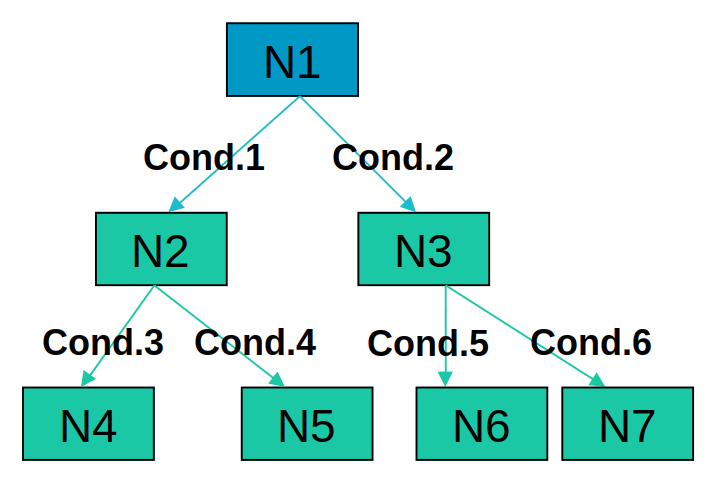
\includegraphics[width=\textwidth]{figs/tree1.png}
             \end{center}
        \end{column}
        \end{columns}
\end{frame}

\begin{frame}{Beslutsträd Exempel}
    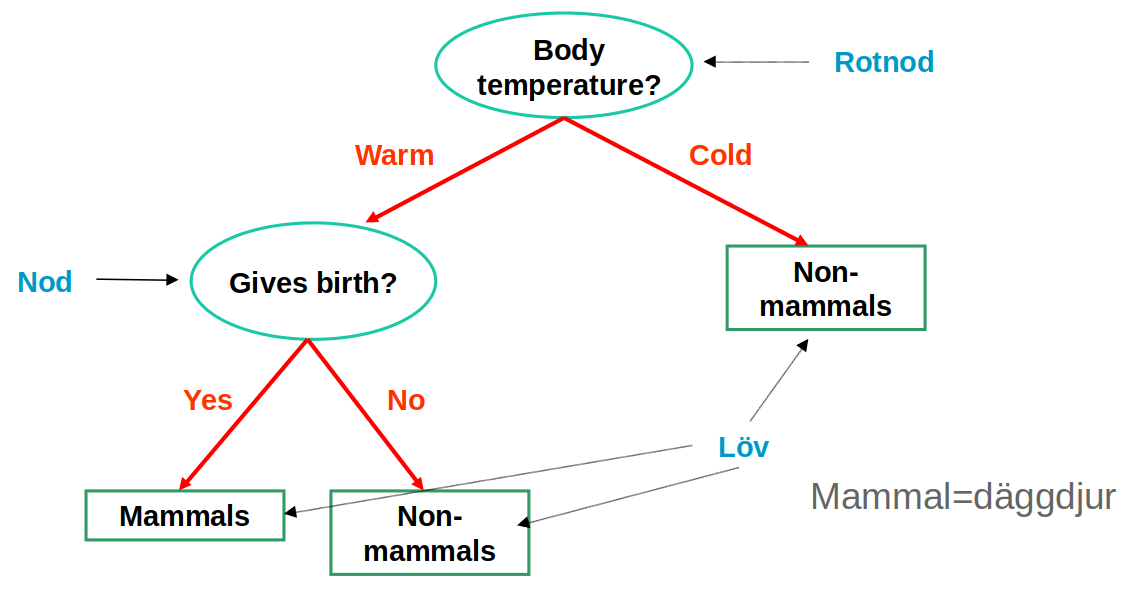
\includegraphics[width=\textwidth]{figs/tree2.png}
\end{frame}

\begin{frame}{Att bygga ett träd}
    \myheading{Hunt's algoritm}
    \begin{enumerate}
        \item Givet en nuvarande datamängd $D_t = \{(X_i, Y_i), i = 1,\ldots,n\}$ för den aktuella noden $t$.
        \item Om alla $Y_i$ är lika, markera $t$ som ett löv och ge värdet $Y_i$.
        \item Annars, använd en \myheading{testregel} för att dela upp $D_t$ i flera delar $D_{t_1}, \ldots, D_{t_k}$ och kör algoritmen (steg 1) för alla dessa noder.
    \end{enumerate}
    
    Denna approach kallas för \textit{recursive binary splitting}.
      
    \myheading{Testregler:}
    \begin{description}
        \item[Binära attribut] Binär uppdelning
        \item[Nomiala attribut] Binär eller mångfaldig uppdelninig
        \item[Ordinala attribut] Uppdelning som bevarar attributsföljden
        \item[Intervall attribut] Uppdelning till icke-överlappande intervall
    \end{description}
\end{frame}

\begin{frame}{Att bygga ett träd - Exempel}

    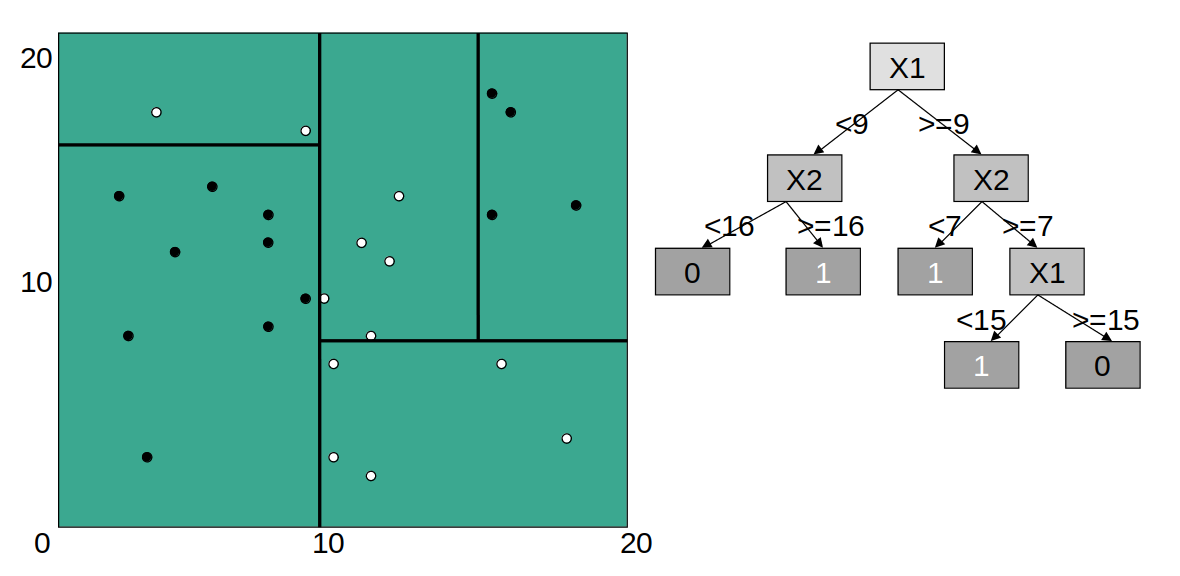
\includegraphics[width=\textwidth]{figs/tree3.png}
    
\end{frame}

\begin{frame}{Trädmodeller}
    
    Sammanfattninig:
    \begin{itemize}
        \item Idé: Dela upp observationerna för att separera klasser.
        \item Uppdelningen sker genom att jämföra testregler.
        \item För att avsluta processen:
        \begin{itemize}
            \item Dela upp tills alla observationer har samma klass
            \item Alt 1. Dela upp tills alla attribut är lika.
            \item Alt 2. Bestäm en regel för tidigt avslut.
        \end{itemize}
    \end{itemize}

\end{frame}

\begin{frame}{CART}
    Classification and Regression Trees (CART).

    I grunden Hunt's algoritm.

    Stöd för kontinuerliga och diskreta utfall.

    Optimering för att välja bästa splitten.
\end{frame}

\begin{frame}{CART - Regressionsträd}
    
    Att försöka minimera RSS över alla möjliga partitioneringar och funktionsvärden är orimligt.

    Istället kör vi med en girig algoritm, där vi vill hitta bästa variabeln $x_j$ och uppdelning $s$ genom att lösa följande problem:
    \begin{align*}
        \min_{j,s} \left[ \min_{c_1} \sum_{x_1 \in R_1(j,s)} (y_i - c_1)^2 + \min_{c_2} \sum_{x_i \in R_2(j,s)} (y_i - c_2)^2 \right], \\
        R_1(j,s) = \{x \mid x_j < s\} \qquad R_2(j,s) = \{x | x_j \geq s\},
    \end{align*}
    $c_1$ och $c_2$ skattas oftast som medelvärdet av respektive region.
\end{frame}

\begin{frame}{CART - Regressionsträd}
    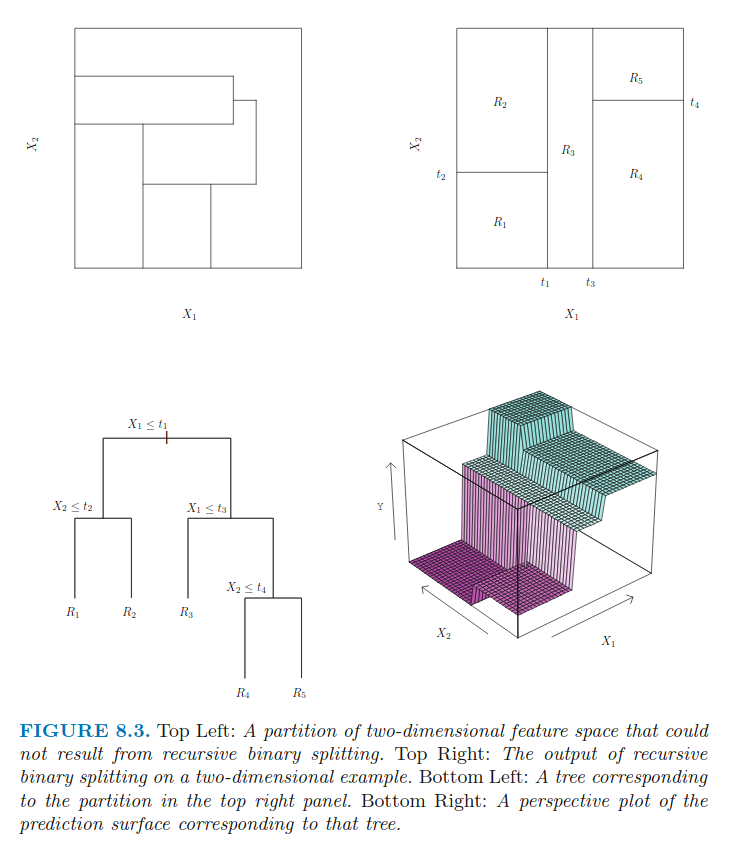
\includegraphics[width=0.68\textwidth]{figs/reg_tree_surface.png}
\end{frame}

\begin{frame}{CART - Klassificeringsträd}
    
    När det kommer till klassificering behöver vi ett nytt mått för att utvärdera om en regel är bra eller dålig.

    Låt $p_{m,k} = \frac{1}{s} \sum_{i : x_i \in R_m} \mathbb{I}_{y_i = k}$ vara proportionen av träningsdata i region $m$ som tillhör klass $k$.

    Kriterier för att välja regioner:
    \begin{description}
        \item[Felkvot] $E = 1 - \max_{k} (p_{m,k})$
        \item[Gini index] $G = \sum_{k} p_{m,k} ( 1 - p_{m,k}) = 1 - \sum_{k} p_{m,k}^2$
        \item[Cross-entropy] $D = - \sum_{k} p_{m,k} \log(p_{m,k})$   
    \end{description}

\end{frame}

\begin{frame}{CART - Klassificeringsträd}

    Välj nu den uppdelning som maximerar informationsvinsten
    \begin{align*}
        \Delta = I(\text{förälder}) - I(\text{barn}), \\
        \Delta = I(\text{förälder}) - \sum_{j} \frac{N(R_j)}{N} I(R_j),
    \end{align*}
    Där
    \begin{description}
        \item[$I(\cdot)$] är ditt valda mått (Felkvot, Gini, Entropy)
        \item[$N$] antal objekt i föräldranoden
        \item[$R_j$] är barnnod $j$
        \item[$N(R_j)$] antal objekt i barnnod $j$    
    \end{description}
    
\end{frame}

\begin{frame}{CART - Klassificeringsträd}

    Predikationer görs med majoritetsröstninig. Vi vill helst att alla observationer i ett löv ska ha samma klass.

    Vi stoppar utbyggnadet på samma sätt som i Hunt's algoritm.

    Entropy och Gini är bättre mått, de ger renare löv.

    Felkvoten används ofta för att utvärdera trädet på testdata.

    Trädmodeller överanpassar väldigt lätt. Vilket ger en hög varians!
    
\end{frame}

\begin{frame}{Motverka överanpassning}

    Viktiga hyperparametrar:
    \begin{itemize}
      \item Trädets djup
      \item Minsta antal obs i en lövnod alt. minsta antal obs i en nod för att överväga en split av noden
    \end{itemize}

    Två olika sätt:
    \begin{description}
        \item[Förbeskärnining]
        \begin{itemize}
            \item Sluta expandera trädet när informationsvinsten är lägre än en vald tröskel.
            \item Kräv ett visst minsta antal obs i varje löv.
        \end{itemize}
        \item[Efterbeskärninig]
        \begin{itemize}
            \item Beskär ett helt utväxt träd, ersätt delträd med ett löv.
        \end{itemize}
    \end{description}
    
\end{frame}

\begin{frame}{Efterbeskärning}
    Använd CART för att ta växa fram ett stort träd $T_0$ på all träningsdata.

    För varje $\alpha \geq 0$ finns ett delträd $T \subset T_0$ som minimerar kostanden
    \begin{equation*}
        C_{\alpha}(T) = \sum_{R \in \text{Löv i T}} N(R) \cdot I(R) + \alpha |T|,
    \end{equation*} 
    där $|T|$ är antalet löv i $T$, $N(R_j)$ antal objekt i lövnod $j$.

    Använd korsvalidering för att skatta $\alpha$, välj det som ger minst valideringsfel.

    Idén är lik LASSO.
\end{frame}

\begin{frame}{Regressionsträd med cost complexity pruning}
    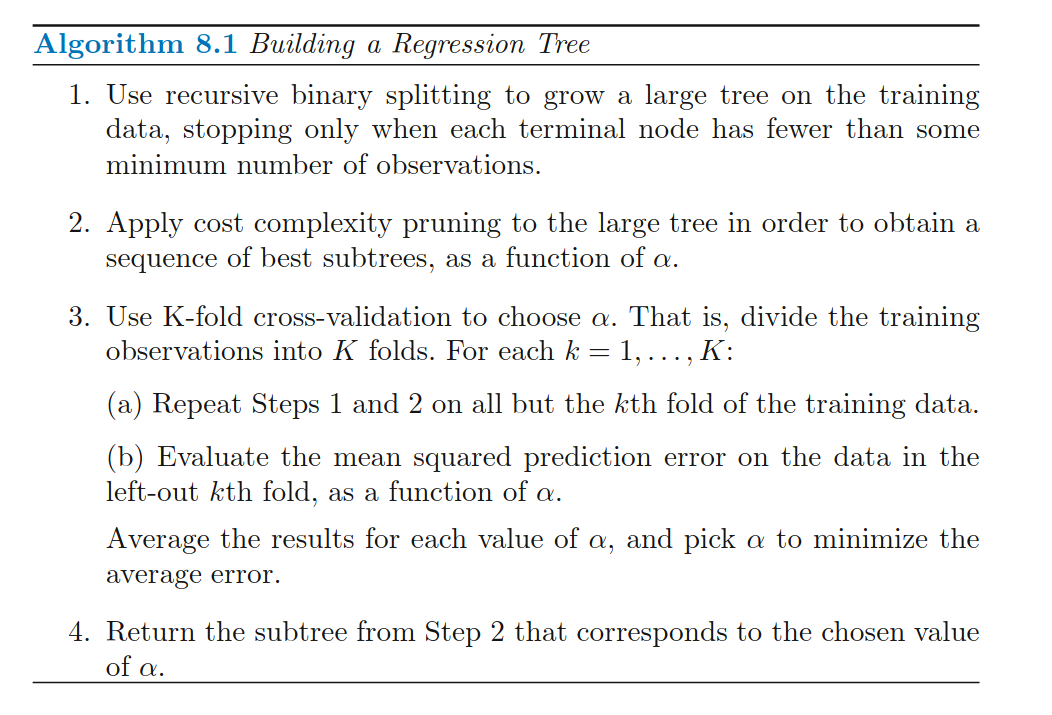
\includegraphics[height=0.9\textheight]{figs/reg_tree_estimate.png}
\end{frame}

\begin{frame}{Trädmodell eller linjär modell}
    För regression har vi:

    \myheading{Linjär regression}
    \begin{equation*}
        f(x) = \beta_0 + \sum_{i=1}^{p} x_i \beta_i
    \end{equation*}

    \myheading{Regressionsträd}
    \begin{equation*}
        f(x) = \sum_{i=1}^{M}c_i \mathbb{I}_{c \in R_i}
    \end{equation*}
\end{frame}

\begin{frame}{Trädmodell eller linjär modell}
    För klassificering har vi:

    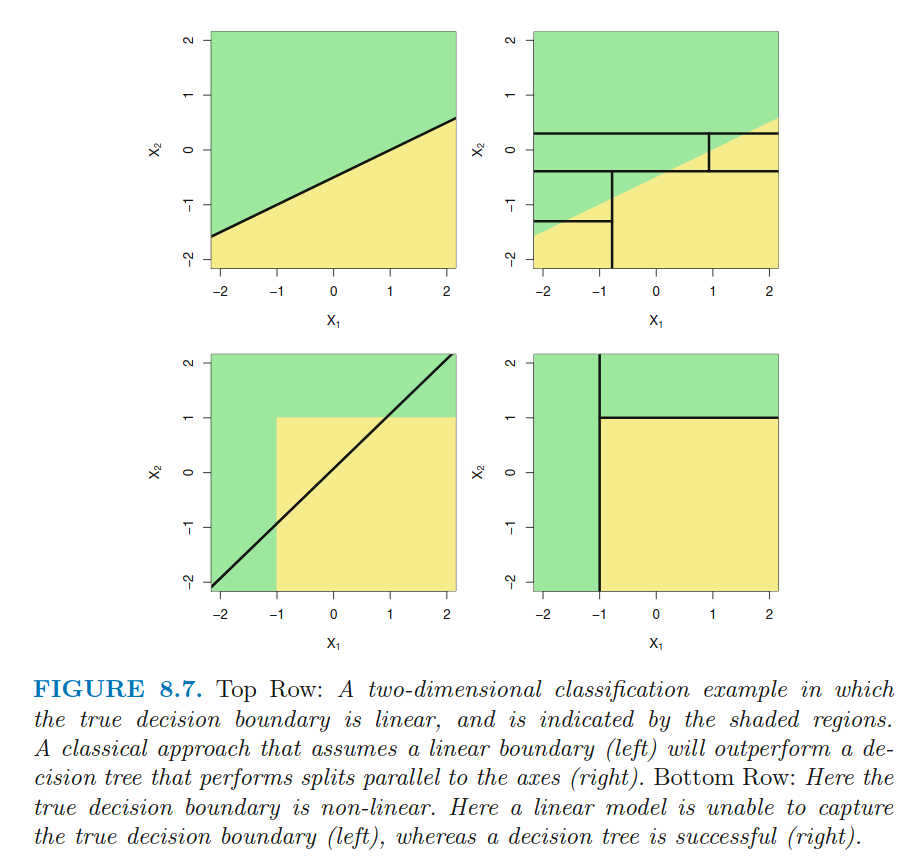
\includegraphics[width=0.68\textwidth]{figs/trees_vs_linear.png}

\end{frame}

\begin{frame}{Kommentarer om trädmodeller}
    Fördelar:
    \begin{itemize}
        \item Lätta att förstå och tolka
        \item Klarar av olika responsvariabler
        \item Kräver inte så mycket datahantering innan
        \item Funkar på relativt stora dataset
        \item Icke-parametrisk metod
        \item Automatisk variabelselektion
        \item Lär sig variabelinteraktioner automatiskt
        \item Kan anpassa många olika sorters funktioner
    \end{itemize}

\end{frame}


\begin{frame}{Kommentarer om trädmodeller}

    Nackdelar:
    \begin{itemize}
        \item Sämre prediktiv förmåga än vissa andra metoder
        \item Orubusta: överanpassar lätt
        \item Omöjligt att hitta det optimala trädet
        \item Vissa enkla funktioner kräver ett komplext träd
    \end{itemize}
\end{frame}



\begin{frame}{Kommentarer om trädmodeller}

    Förbättringar:
    \begin{itemize}
        \item Bagging
        \item Random forest
        \item Boosting
        \item BART: Bayesian Additive Regression Trees
    \end{itemize}
    
\end{frame}

\end{document}